\documentclass[border=10pt]{standalone}
\usepackage{tikz}
\usepackage{amsmath}
\begin{document}
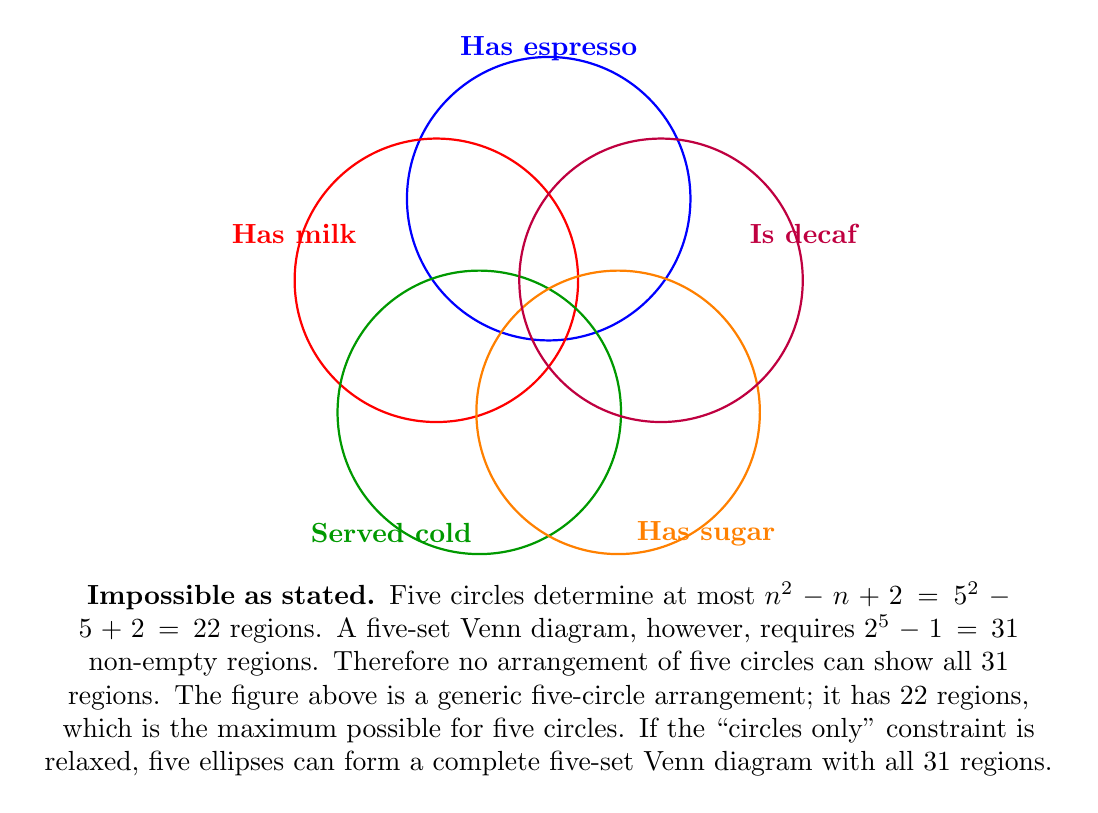
\begin{tikzpicture}[scale=1.0]
  % Five congruent circles whose centres form a regular pentagon.
  % Let R = 1.5 (pentagon circumradius) and r = 1.8 (circle radius).
  % R is not equal to r, so no three circles meet in one point.
  % Every pair of circles intersects, giving the maximum 22 regions.
  \draw[thick, blue]            (90:1.5)  circle (1.8);
  \draw[thick, red]             (162:1.5) circle (1.8);
  \draw[thick, green!60!black]  (234:1.5) circle (1.8);
  \draw[thick, orange]          (306:1.5) circle (1.8);
  \draw[thick, purple]          (18:1.5)  circle (1.8);

  % Labels placed on the outer edge of each circle.
  \node[blue, font=\bfseries]            at (90:3.4)  {Has espresso};
  \node[red, font=\bfseries]             at (162:3.4) {Has milk};
  \node[green!60!black, font=\bfseries]  at (234:3.4) {Served cold};
  \node[orange, font=\bfseries]          at (306:3.4) {Has sugar};
  \node[purple, font=\bfseries]          at (18:3.4)  {Is decaf};

  % Explanation: 31 regions is impossible with circles.
  \node[align=center, text width=13cm] at (0,-4.6) {
    \textbf{Impossible as stated.}  Five circles determine at most
    $n^2-n+2 = 5^2-5+2 = 22$ regions.  A five-set Venn diagram,
    however, requires $2^5-1 = 31$ non-empty regions.  Therefore
    no arrangement of five circles can show all 31 regions.
    The figure above is a generic five-circle arrangement; it has
    22 regions, which is the maximum possible for five circles.
    If the ``circles only'' constraint is relaxed, five ellipses can
    form a complete five-set Venn diagram with all 31 regions.
  };
\end{tikzpicture}
\end{document}
